%% автогенерация: scripts/figures_tex.py — руками не править
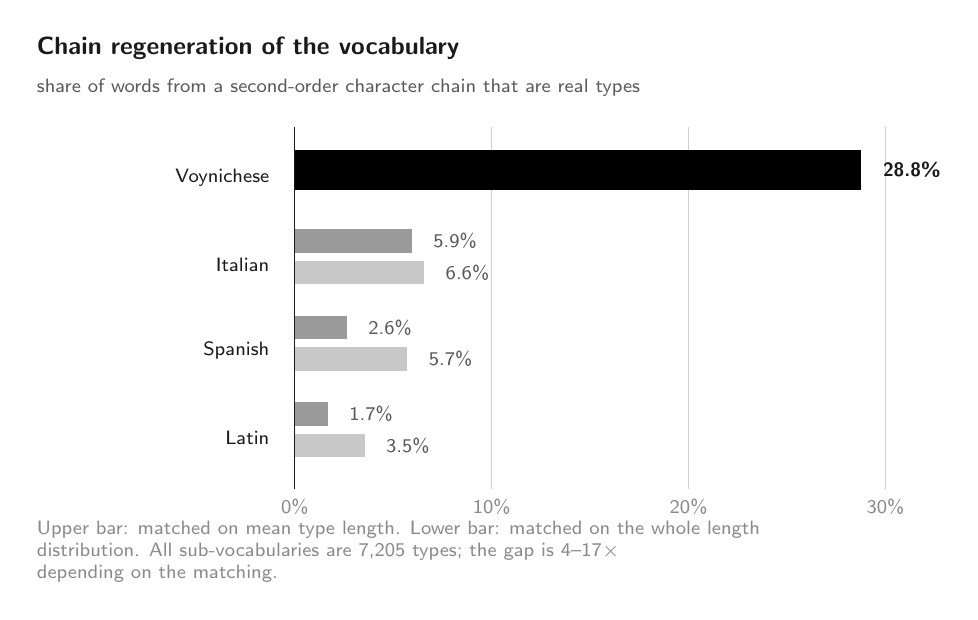
\begin{tikzpicture}[x=1mm,y=1mm,font=\sffamily\scriptsize]
\definecolor{ink}{HTML}{1A1A1A}\definecolor{inkii}{HTML}{5A5A5A}
\definecolor{inkiii}{HTML}{8A8A8A}\definecolor{rule}{HTML}{D0D0D0}
\definecolor{fill}{HTML}{2B2B2B}\definecolor{fillii}{HTML}{9A9A9A}
\definecolor{filliii}{HTML}{C8C8C8}
\node[anchor=west,font=\sffamily\small\bfseries,text=ink] at (0,57) {Chain regeneration of the vocabulary};
\node[anchor=west,text=inkii] at (0,52) {share of words from a second-order character chain that are real types};
\draw[ink] (34.0,47) -- (34.0,1);
\node[below,text=inkiii] at (34.0,1) {0\%};
\draw[rule] (59.0,47) -- (59.0,1);
\node[below,text=inkiii] at (59.0,1) {10\%};
\draw[rule] (84.0,47) -- (84.0,1);
\node[below,text=inkiii] at (84.0,1) {20\%};
\draw[rule] (109.0,47) -- (109.0,1);
\node[below,text=inkiii] at (109.0,1) {30\%};
\node[anchor=east,text=ink] at (32,40.5) {Voynichese};
\fill[fill] (34,39) rectangle (105.96391394864678,44);
\node[anchor=west,font=\sffamily\scriptsize\bfseries,text=ink] at (107.46391394864678,41.5) {28.8\%};
\node[anchor=east,text=ink] at (32,29.5) {Italian};
\fill[fillii] (34,31) rectangle (48.853111265325005,34);
\fill[filliii] (34,27) rectangle (50.42170586039567,30);
\node[anchor=west,text=inkii] at (50.353111265325005,32.5) {5.9\%};
\node[anchor=west,text=inkii] at (51.92170586039567,28.5) {6.6\%};
\node[anchor=east,text=ink] at (32,18.5) {Spanish};
\fill[fillii] (34,20) rectangle (40.597270414064305,23);
\fill[filliii] (34,16) rectangle (48.27309908905001,19);
\node[anchor=west,text=inkii] at (42.097270414064305,21.5) {2.6\%};
\node[anchor=west,text=inkii] at (49.77309908905001,17.5) {5.7\%};
\node[anchor=east,text=ink] at (32,7.5) {Latin};
\fill[fillii] (34,9) rectangle (38.189220448762434,12);
\fill[filliii] (34,5) rectangle (42.85751560898332,8);
\node[anchor=west,text=inkii] at (39.689220448762434,10.5) {1.7\%};
\node[anchor=west,text=inkii] at (44.35751560898332,6.5) {3.5\%};
\node[anchor=west,text=inkiii,align=left] at (0,-7) {Upper bar: matched on mean type length. Lower bar: matched on the whole length\\distribution. All sub-vocabularies are 7,205 types; the gap is 4--17$\times$\\depending on the matching.};
\end{tikzpicture}
